\documentclass[twoside,twocolumn]{article}

\usepackage{blindtext} 
\usepackage{graphicx}
\usepackage[sc]{mathpazo} 
\usepackage[T1]{fontenc} 
\linespread{1.05} 
\usepackage{microtype} 


\usepackage[english]{babel} 


\usepackage[hmarginratio=1:1,top=32mm,columnsep=20pt]{geometry} 
\usepackage[hang, small,labelfont=bf,up,textfont=it,up]{caption} 
\usepackage{booktabs} 


\usepackage{lettrine} 


\usepackage{enumitem} 
\setlist[itemize]{noitemsep} 


\usepackage{abstract} 
\renewcommand{\abstractnamefont}{\normalfont\bfseries} 
\renewcommand{\abstracttextfont}{\normalfont\small\itshape} 


\usepackage{titlesec} 
\renewcommand\thesection{\Roman{section}} % 
\renewcommand\thesubsection{\roman{subsection}} 
\titleformat{\section}[block]{\large\scshape\centering}{\thesection.}{1em}{} 
\titleformat{\subsection}[block]{\large}{\thesubsection.}{1em}{} 


\usepackage{fancyhdr} 
\pagestyle{fancy} 
\fancyhead{} 
\fancyfoot{} 
\fancyhead[C]{Balanced ScoreCard y Business Model Canvas $\bullet$ Septiembre 2019 $\bullet$ } 
\fancyfoot[RO,LE]{\thepage} 


\usepackage{titling} 


\usepackage{hyperref} 


%----------------------------------------------------------------------------------------
%	TILULOS
%----------------------------------------------------------------------------------------


\setlength{\droptitle}{-4\baselineskip} 

\pretitle{\begin{center}\Huge\bfseries} 
\posttitle{\end{center}} 
\title{Inmon vs Kimball} 
\author{Andre Sebastian Reinoso Aranda\\
}
\date{\today} 
\renewcommand{\maketitlehookd}{

\begin{abstract}
\noindent 
Un Data WareHouse, almacen de datos, una coleccion de datos aorientada a un determinado contexto y ambito (empresas, instituciones, organizaciones, etc.). integro, no volatil y que puede cambiar en el tiempo. El principal objetivo es el de ayudar a las empresas, instituciones, organizaciones, etc. Que ayuda a tomar decisiones en la entidad quien la utilizara. Siempre a base del historial de las operaciones de la entidad que son almacenadas en una base de datos diseñada a favorecer el analisis, propagacion de los datos, con herramientas.
Por lo general las empresas medianas y grandes los datos provienen de diferentes sistemas que posee la entidad y lo que busca el Data WareHouse es unificarlas y poder operar sobre ellas con la finalidad de buscar la buena toma de decisiones.

\end{abstract}


\begin{abstract}
\noindent 
A Data WareHouse,a collection of data oriented to a certain context and scope (companies, institutions, organizations, etc.). Integral, not volatile and that can change over time. The main objective is to help companies, institutions, organizations, etc. That helps to make decisions in the entity that will use it. Always based on the history of the operations of the entity that are stored in a database designed to favor the analysis, the propagation of the data, with tools.
In general, medium and large companies, the data comes from different systems that the entity has and what Data WareHouse seeks is to unify and operate in them to seek a good decision making.
\end{abstract}
}

%----------------------------------------------------------------------------------------

\begin{document}

% Print the title
\maketitle

%----------------------------------------------------------------------------------------
%	INTRODUCCION
%----------------------------------------------------------------------------------------

\section{Introduccion}
\lettrine[nindent=0em,lines=3]{E}n la actualidad el mundo de los negocios plantea la necesidad de disponer de un acceso rápido y sencillo a información para la toma de decisiones. Dicha información debe estar estructurada y elaborada de acuerdo a parámetros de calidad, a fin de posibilitar una adaptación ágil y precisa a las fluctuaciones del ambiente externo.
Los niveles gerenciales necesitan a menudo tomar decisiones de alto nivel, cruciales para el funcionamiento de la empresa. Frecuentemente se basan en su experiencia este enfoque no es apto para las condiciones del mundo actual en el que los sistemas de gestión de calidad vigentes han demostrado la importancia de la toma de decisiones basada en cifras, datos y hechos. El Data Warehouse permite que los gerentes tomen decisiones siguiendo un enfoque racional, basados en información confiable y oportuna. Es tarea fundamental del Data Warehouse recolectar, unificar y depurar los datos del negocio, eliminando inconsistencias y conservando sólo la información útil para los objetivos empresariales.



%----------------------------------------------------------------------------------------
%	Objetivos
%----------------------------------------------------------------------------------------


\section{Objetivos}

\begin{itemize}
\item Entender la importancia del Data WareHouse en las empresas, orgnizaciones, entidades, instituciones, etc.
\item Desarrollar los antecedentes de las metodologias descritas por William H. Inmon y Ralph Kimball.
\item Comparativo de las metodologias descritas por William H. Inmon y Ralph Kimball.

\end{itemize}


%----------------------------------------------------------------------------------------
%	Marco teorico
%----------------------------------------------------------------------------------------


\section{Antecedentes}

\begin{enumerate}

 \item \textbf{William H. Inmon}
\\
William H. Inmon, científico informático estadounidense, reconocido por muchos como el padre del Data WareHouse Inmon escribió el primer libro, celebró la primera conferencia, escribió la primera columna en una revista y fue el primero en ofrecer clases del Data WareHouse. Inmon creó la definición aceptada de lo que es un Data WareHouse: una recopilación de datos variada de tiempo, no volátil, integrada y orientada al tema, en apoyo de las decisiones de la gerencia. En comparación con el enfoque del otro arquitecto pionero del almacenamiento de datos, Ralph Kimball, el enfoque de Inmon a menudo se caracteriza como un enfoque de arriba hacia abajo.
\\ 

\item \textbf{Ralph Kimball}
\\
Ralph Kimball  un autor sobre el tema del almacenamiento de datos y la inteligencia empresarial. Es uno de los arquitectos originales del almacenamiento de datos y es conocido por sus convicciones a largo plazo de que los almacenes de datos deben estar diseñados para ser comprensibles y rápidos. Su metodología, también conocida como modelado dimensional o la metodología Kimball, se ha convertido en el estándar de facto en el área de soporte de decisiones.

\end{enumerate}

%----------------------------------------------------------------------------------------
%	DESAROLLO
%----------------------------------------------------------------------------------------

\section{DESARROLLO}
\begin{enumerate}
 \item \textbf{¿Que es un Data Warehouse?}\\
Area de almacenamiento donde todos los datos de la empresa se guardan en un solo lugar. Esto incluye datos de diferentes fuentes, así como datos actuales e históricos, tal vez de una plataforma heredada.\\ \\
Puede consistir en datos de la propia empresa, que si la empresa es grande podría extenderse a muchos departamentos, todos los cuales pueden estar utilizando diferentes formatos y diferentes plataformas. Sin mencionar los datos de fuentes externas, ya sea de otras empresas o de contenido generado por el usuario.[2]

 \item \textbf{¿Que es un Data Mart?} \\
Estructura de datos, construido dentro de una base de datos este almacena información agregada o consolidada, que será consumida por alguna herramienta de visualización o data analytics. generalmente Datamart se especializa en un área de la empresa o de un flujo o proceso especifico. \\

Un Datamart almacenara la información proveniente de uno o más orígenes de datos (bases de datos, archivos con datos, servicios de internet, etc.) y que ha sido procesada por un ETL (proceso de Extracción, Transformación y Carga).\\

El Datamart contiene información consolidada, se actualiza periódicamente.

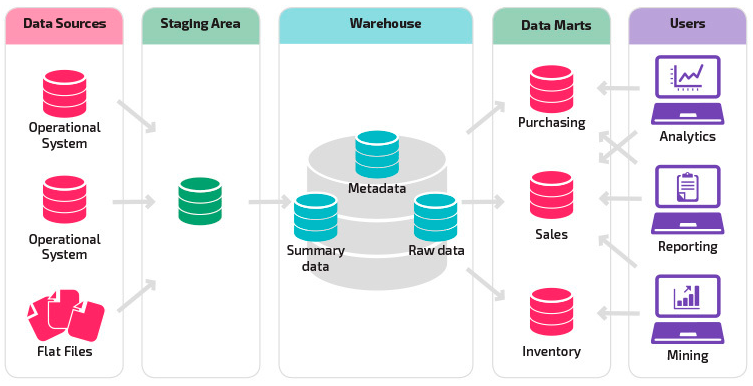
\includegraphics[width=7cm, height=5cm]{Imagenes/datawarehouse_datamart}

 \item \textbf{Enfoque Inmon}

Bill Inmon ve la necesidad de transferir la información de los diferentes OLTP (Sistemas Transaccionales) de las organizaciones a un lugar centralizado donde los datos puedan ser utilizados para el analisis (sería el CIF o Corporate Information Factory).\\

Insiste ademas en que ha de tener las siguientes características:

\textbf{Orientado a temas} Los datos en la base de datos están organizados de manera que todos los elementos de datos relativos al mismo evento u objeto del mundo real queden unidos entre sí.
\\ \\
\textbf{Integrado} La base de datos contiene los datos de todos los sistemas operacionales de la organización, y dichos datos deben ser consistentes.
\\ \\
\textbf{No volátil} La información no se modifica ni se elimina, una vez almacenado un dato, éste se convierte en información de sólo lectura, y se mantiene para futuras consultas.
\\ \\
\textbf{Variante en el tiempo} Los cambios producidos en los datos a lo largo del tiempo quedan registrados para que los informes que se puedan generar reflejen esas variaciones.
\\ \\
La información ha de estar a los máximos niveles de detalle. Los Dw departamentales o datamarts son tratados como subconjuntos de este Dw corporativo, que son construidos para cubrir las necesidades individuales de analisis de cada departamento, y siempre a partir de este Dw Central (del que también se pueden construir los ODS ( Operational Data Stores ) o similares).

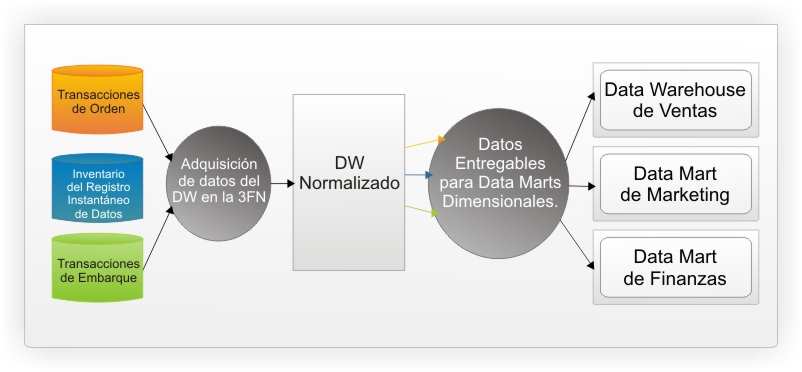
\includegraphics[width=7cm, height=5cm]{Imagenes/enfoque-inmon}

 \item \textbf{Enfoque Kimball}

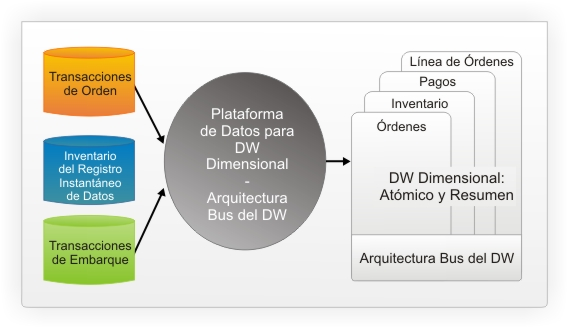
\includegraphics[width=7cm, height=5cm]{Imagenes/enfoque-kimball}
   
\end{enumerate}


%----------------------------------------------------------------------------------------
%	GRAFICOS
%----------------------------------------------------------------------------------------

\section{graficos}
\begin{enumerate}

 \item Uno
   
\end{enumerate}

%----------------------------------------------------------------------------------------
%	DIAGRAMAS
%----------------------------------------------------------------------------------------

\section{Análisis}

\begin{enumerate}

    \item Uno
\end{enumerate}

%----------------------------------------------------------------------------------------
%	CONCLUSIONES
%----------------------------------------------------------------------------------------

\section{Conclusiones}
\begin{itemize}	
 \item Uno

\end{itemize} 



%----------------------------------------------------------------------------------------
%	BIBLIOGRAFIA
%----------------------------------------------------------------------------------------


\begin{thebibliography}{99} 

\bibitem[1]{}
\newblock W. H. Inom, 2002. Building the Data Warehouse

\bibitem[2]{}
\newblock Spotless. Exploring Data Warehouse and Data Quality, Reduperado de: web.archive.org

\bibitem[3]{}
\newblock I, Abramson, 20 IAS Inc. Data Warehouse: The Choice of Inmon versus Kimball

\end{thebibliography}


%----------------------------------------------------------------------------------------


\end{document}
